\documentclass[12pt,letterpaper,oneside,reqno]{amsart}
\usepackage{amsfonts}
\usepackage{amsmath}
\usepackage{amssymb}
\usepackage{amsthm}
\usepackage{float}
\usepackage{mathrsfs}
\usepackage{colonequals}
\usepackage[font=small,labelfont=bf]{caption}
\usepackage[left=1in,right=1in,bottom=1in,top=1in]{geometry}
\usepackage[pdfpagelabels,hyperindex,colorlinks=true,linkcolor=blue,urlcolor=magenta,citecolor=green]{hyperref}
\usepackage{graphicx}
\linespread{1.7}
\emergencystretch=1em
\usepackage{array}
\usepackage{etoolbox}
\apptocmd{\sloppy}{\hbadness 10000\relax}{}{}
\raggedbottom

\newcommand \anglePower [2]{\langle #1 \rangle \sp{#2}}
\newcommand \bernoulli [2][B] {{#1}\sb{#2}}
\newcommand \curvePower [2]{\{#1\}\sp{#2}}
\newcommand \coeffA [3][A] {{\mathbf{#1}} \sb{#2,#3}}
\newcommand \polynomialP [4][P]{{\mathbf{#1}}\sp{#2} \sb{#3}(#4)}

% ordinary derivatives
\newcommand \derivative [2] {\frac{d}{d #2} #1}                              % 1 - function; 2 - variable;
\newcommand \pderivative [2] {\frac{\partial #1}{\partial #2}}               % 1 - function; 2 - variable;
\newcommand \qderivative [1] {D_{q} #1}                                      % 1 - function
\newcommand \nqderivative [1] {D_{n,q} #1}                                   % 1 - function
\newcommand \qpowerDerivative [1] {\mathcal{D}_q #1}                         % 1 - function;
\newcommand \finiteDifference [1] {\Delta #1}                                % 1 - function;
\newcommand \pTsDerivative [2] {\frac{\partial #1}{\Delta #2}}               % 1 - function; 2 - variable;

% high order derivatives
\newcommand \derivativeHO [3] {\frac{d^{#3}}{d {#2}^{#3}} #1}                % 1 - function; 2 - variable; 3 - order
\newcommand \pderivativeHO [3]{\frac{\partial^{#3}}{\partial {#2}^{#3}} #1}
\newcommand \qderivativeHO [2] {D_{q}^{#2} #1}                               % 1 - function; 2 - order
\newcommand \qpowerDerivativeHO [2] {\mathcal{D}_{q}^{#2} #1}                % 1 - function; 2 - order
\newcommand \finiteDifferenceHO [2] {\Delta^{#2} #1}                         % 1 - function; 2 - order
\newcommand \pTsDerivativeHO [3] {\frac{\partial^{#3}}{\Delta {#2}^{#3}} #1} % 1 - function; 2 - variable;

\newtheorem{thm}{Theorem}[section]
\newtheorem{cor}[thm]{Corollary}
\newtheorem{lem}[thm]{Lemma}
\newtheorem{examp}[thm]{Example}
\newtheorem{conj}[thm]{Conjecture}
\newtheorem{defn}[thm]{Definition}

\numberwithin{equation}{section}

\title[On the summation of divergent series]
{On the summation of divergent series}
\author[Petro Kolosov]{Petro Kolosov}
\email{kolosovp94@gmail.com}
\keywords{
    Ramanujan summation, divergent series
}
\urladdr{https://kolosovpetro.github.io}
\subjclass[2010]{26E70, 05A30}
\date{\today}
\hypersetup{
    pdftitle={On the summation of divergent series},
    pdfsubject={
        Ramanujan summation, divergent series
    },
    pdfauthor={Petro Kolosov},
    pdfkeywords={
        Ramanujan summation, divergent series
    }
}
\begin{document}
    \begin{abstract}
        Your abstract here.
    \end{abstract}

    \maketitle

    \tableofcontents


    \section{Introduction} \label{sec:introduction}
    Your introduction here.
Include some references~\cite{bayour2017truly,benkhettou2016conformable,caputo2009time,martins2009calculus,
    GithubSource_2022, Sloane_theencyclopedia}.
Lorem Ipsum is simply dummy text of the printing and typesetting industry.
Lorem Ipsum has been the industry's standard dummy text ever since the 1500s, when an unknown printer took a galley
of type and scrambled it to make a type specimen book.
It has survived not only five centuries, but also the leap into electronic typesetting, remaining essentially unchanged.
It was popularised in the 1960s with the release of Letraset sheets containing Lorem Ipsum passages, and more
recently with desktop publishing software like Aldus PageMaker including versions of Lorem Ipsum.

Figure example
\begin{figure}[H]
    \centering
    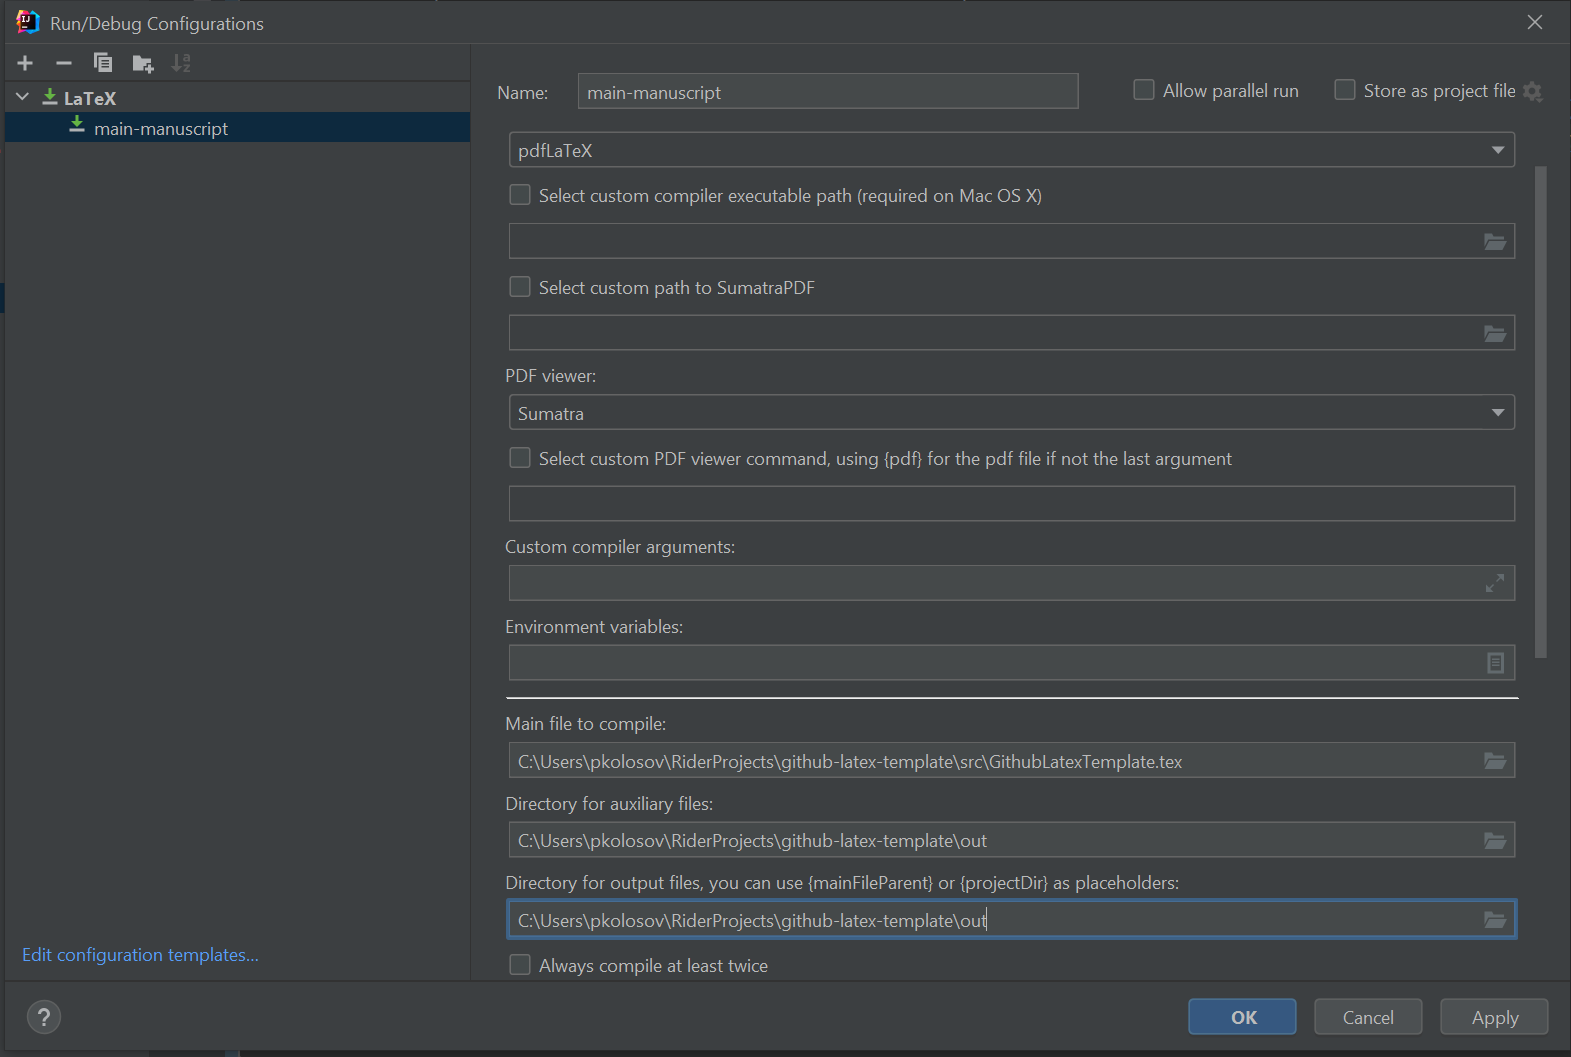
\includegraphics[width=1\textwidth]{../img/latex_configuration}
    ~\caption{Figure example.}\label{fig:figure}
\end{figure}


    \section{Heuristic background}\label{sec:heurisitc-background}
    In chapter 8 of the first collection of his writings, Ramanujan showed that $1+2+3+4+\cdots = \frac{-1}{12}$ using two
methods.
The first key observation is that the series $1+2+3+4+\cdots$ is similar to the alternating series of natural
numbers $1-2+3-4+\cdots$.
Although this series is also divergent, it is much easier to work with.
There are several classical ways to assign a final value to this series, known since the 18th century.

In order to bring the series $1+2+3+4+\cdots$ to the form $1-2+3-4+\cdots$, we can subtract 4 from the second
term, 8 from the fourth term, 12 from the sixth, etc.
The total value to be subtracted is expressed by the series $4+8+12+16+\cdots$, which is obtained by multiplying the
original series $1+2+3+4+\cdots$ by 4.
Let be $c$
\begin{equation*}
    c = 1+2+3+4+\cdots
\end{equation*}
Then $4c$ is
\begin{equation*}
    4c = 4+8+12+16+\cdots
\end{equation*}
If we subtract $4c$ from $c$ we get
\begin{equation}
    -3c = 1-2+3-4+\cdots\label{eq:equation2}
\end{equation}
Here we notice that $1-2+3-4+\cdots$ is Taylor series $T(x)$ of $f(x) = \frac{1}{(1+x)^2}$ for $x=1$, eg
\begin{align*}
    T(x) &= 1 - 2x + 3x^2 - 4x^3 + 5x^4 - 6x^5 + O(x^6) \\
    T(1) &= 1 - 2 + 3 - 4 + 5 - 6 + \cdots
\end{align*}
Therefore, equation (2.1) turns to
\begin{align*}
    -3c = 1-2+3-4+\cdots = \frac{1}{(1 + 1)^2} = \frac{1}{4}
\end{align*}
Finally, the sum of natural series is
\begin{equation*}
    c = 1+2+3+4+\cdots = -\frac{1}{12}.
\end{equation*}
Furthermore, this approach was extended to Ramanujan's summation method, which involves Euler-Maclaurin formula.


    \section{Ramanujan's summation formula}\label{sec:ramanujan's-summation-formula}
    Ramanujan summation essentially is a property of the partial sums, rather than a property of the entire sum,
as that doesn't exist.
If we take the Euler-Maclaurin summation formula together with the correction rule using Bernoulli numbers, we see that
\begin{align*}
    \frac {1}{2}f(0)+f(1)+\cdots +f(n-1)+{\frac {1}{2}}f(n)
    &={\frac {1}{2}}[f(0)+f(n)]+\sum _{k=1}^{n-1}f(k)\\
    &=\int _{0}^{n}f(x)\,dx+\sum _{k=1}^{p}{\frac {B_{k+1}}{(k+1)!}}\left[f^{(k)}(n)-f^{(k)}(0)\right]+R_{p}
\end{align*}
Ramanujan wrote it for the case p going to infinity
\begin{equation*}
    \sum _{k=1}^{x}f(k)=C+\int _{0}^{x}f(t)\,dt+{\frac {1}{2}}f(x)+\sum_{k=1}^{\infty }{\frac {B_{2k}}{(2k)!}}f^{(2k-1)}(x)
\end{equation*}
Therefore, yet again we get a value of natural series equals to $-\frac{1}{12}$
\begin{equation*}
    \sum_{k=1}^{\infty} k =-{\frac {1}{2}}f(0)-\sum _{k=1}^{\infty }{\frac {B_{2k}}{(2k)!}}f^{(2k-1)}(0) = \frac {1}{6}\cdot {\frac {1}{2!}}=-\frac {1}{12}
\end{equation*}


    \section{Riemann zeta function}\label{sec:riemann-zeta-function}
    We continue our journey to the world of divergent series from the one very widely-known formula, it's called a Riemann
zeta function $\zeta(s)$.
For every $s \in \mathbb{R}$ Riemann zeta function is defined as
\begin{equation*}
    \zeta(s) = \sum_{n=1}^{\infty} \frac{1}{n^s}.
\end{equation*}
The following identity holds in terms of zeta function
\begin{equation*}
    \zeta(1 - N) = -\frac{B_N}{N}
\end{equation*}
Consider the case $N=1$
\begin{equation*}
    \sum_{n=1}^{\infty} 1 = \zeta(1 - N)  = - \frac{B_1}{1} = \frac{1}{2}
\end{equation*}
since Bernoulli number $B_1 = \frac{1}{2}$.
Similarly for $N = 2,3$
\begin{align*}
    \sum_{n=1}^{\infty} n &= \zeta(1 - 2) = -\frac{B_2}{2} = -\frac{1}{12} \\
    \sum_{n=1}^{\infty} n^2 &= \zeta(1 - 3) = -\frac{B_3}{3} = 0 \\
    \sum_{n=1}^{\infty} n^3 &= \zeta(1 - 4) = -\frac{B_4}{4} = \frac{1}{120}
\end{align*}

In general,

\begin{equation*}
    \sum_{k=1}^{\infty} k^N = \zeta(1 - N) = -\frac{B_N}{N} = \mathrm{const}
\end{equation*}


    \section{Conclusions}\label{sec:conclusions}
    Conclusions of your manuscript.

%    \bibliographystyle{unsrt}
%    \bibliography{DivergentSeries}
    \noindent \textbf{Version:} \texttt{Local-0.1.0}

\end{document}
